\section{数据来源与预处理}

TCGA是癌症研究领域最重要的公共多组学数据库之一，覆盖大量癌种的基因组、转录组、表观组、蛋白组以及临床信息。数据规模大、注释较完整、样本来源统一，非常适合用于多组学方法研究。UCSC Xena提供TCGA及其他公共项目的统一下载与可视化入口，方便研究者获取不同组学的标准化矩阵和临床标签。本研究采用的TCGA-BRCA数据包含三类核心信息：RNA-seq表达矩阵、DNA甲基化矩阵以及临床亚型标签。RNA和甲基化矩阵均以“特征 × 样本”形式组织，临床标签文件用于提供监督学习的类别标注。

RNA-seq数据在本研究中承担最基础的功能表达信息角色。转录组矩阵记录了每个基因在不同样本中的表达水平，其维度通常较高，且表达分布具有明显偏态：少量高表达基因占据较大信号，而大量低表达基因对分类的贡献有限。因此，RNA预处理通常需要进行对数变换、低表达过滤与高方差特征筛选。当前实现采用log2(TPM + 1)形式进行数值变换，压缩极端值并缓解表达量分布不均问题。随后使用均值过滤与方差排序保留高区分度特征。这个步骤在实验中起到两个作用：一是降低噪声，二是避免模型被大量无关基因拖累。对于高维小样本场景，这类特征筛选往往比复杂的深度模型更稳定。

甲基化数据反映CpG位点上的表观遗传状态，维度更高，典型平台如Illumina 450K可能包含数十万条探针。与RNA不同，甲基化数据的解释通常更偏向调控层面：某些启动子区域的甲基化升高可能导致相关基因沉默，不同亚型在甲基化谱上的差异往往反映调控机制的变化。由于甲基化数据极高维且稀疏，直接进入分类器容易出现严重过拟合。本研究同样采用高方差筛选策略，只保留最具区分度的探针。当前实现中，甲基化预处理先删除缺失值，再按方差排序保留Top-K特征。该策略虽然简单，但在当前中小样本实验中具有较高的可操作性。高方差筛选前后RNA和甲基化特征的分布对比如图~\ref{fig:feature-distribution}所示。

\begin{figure}[H]
\centering
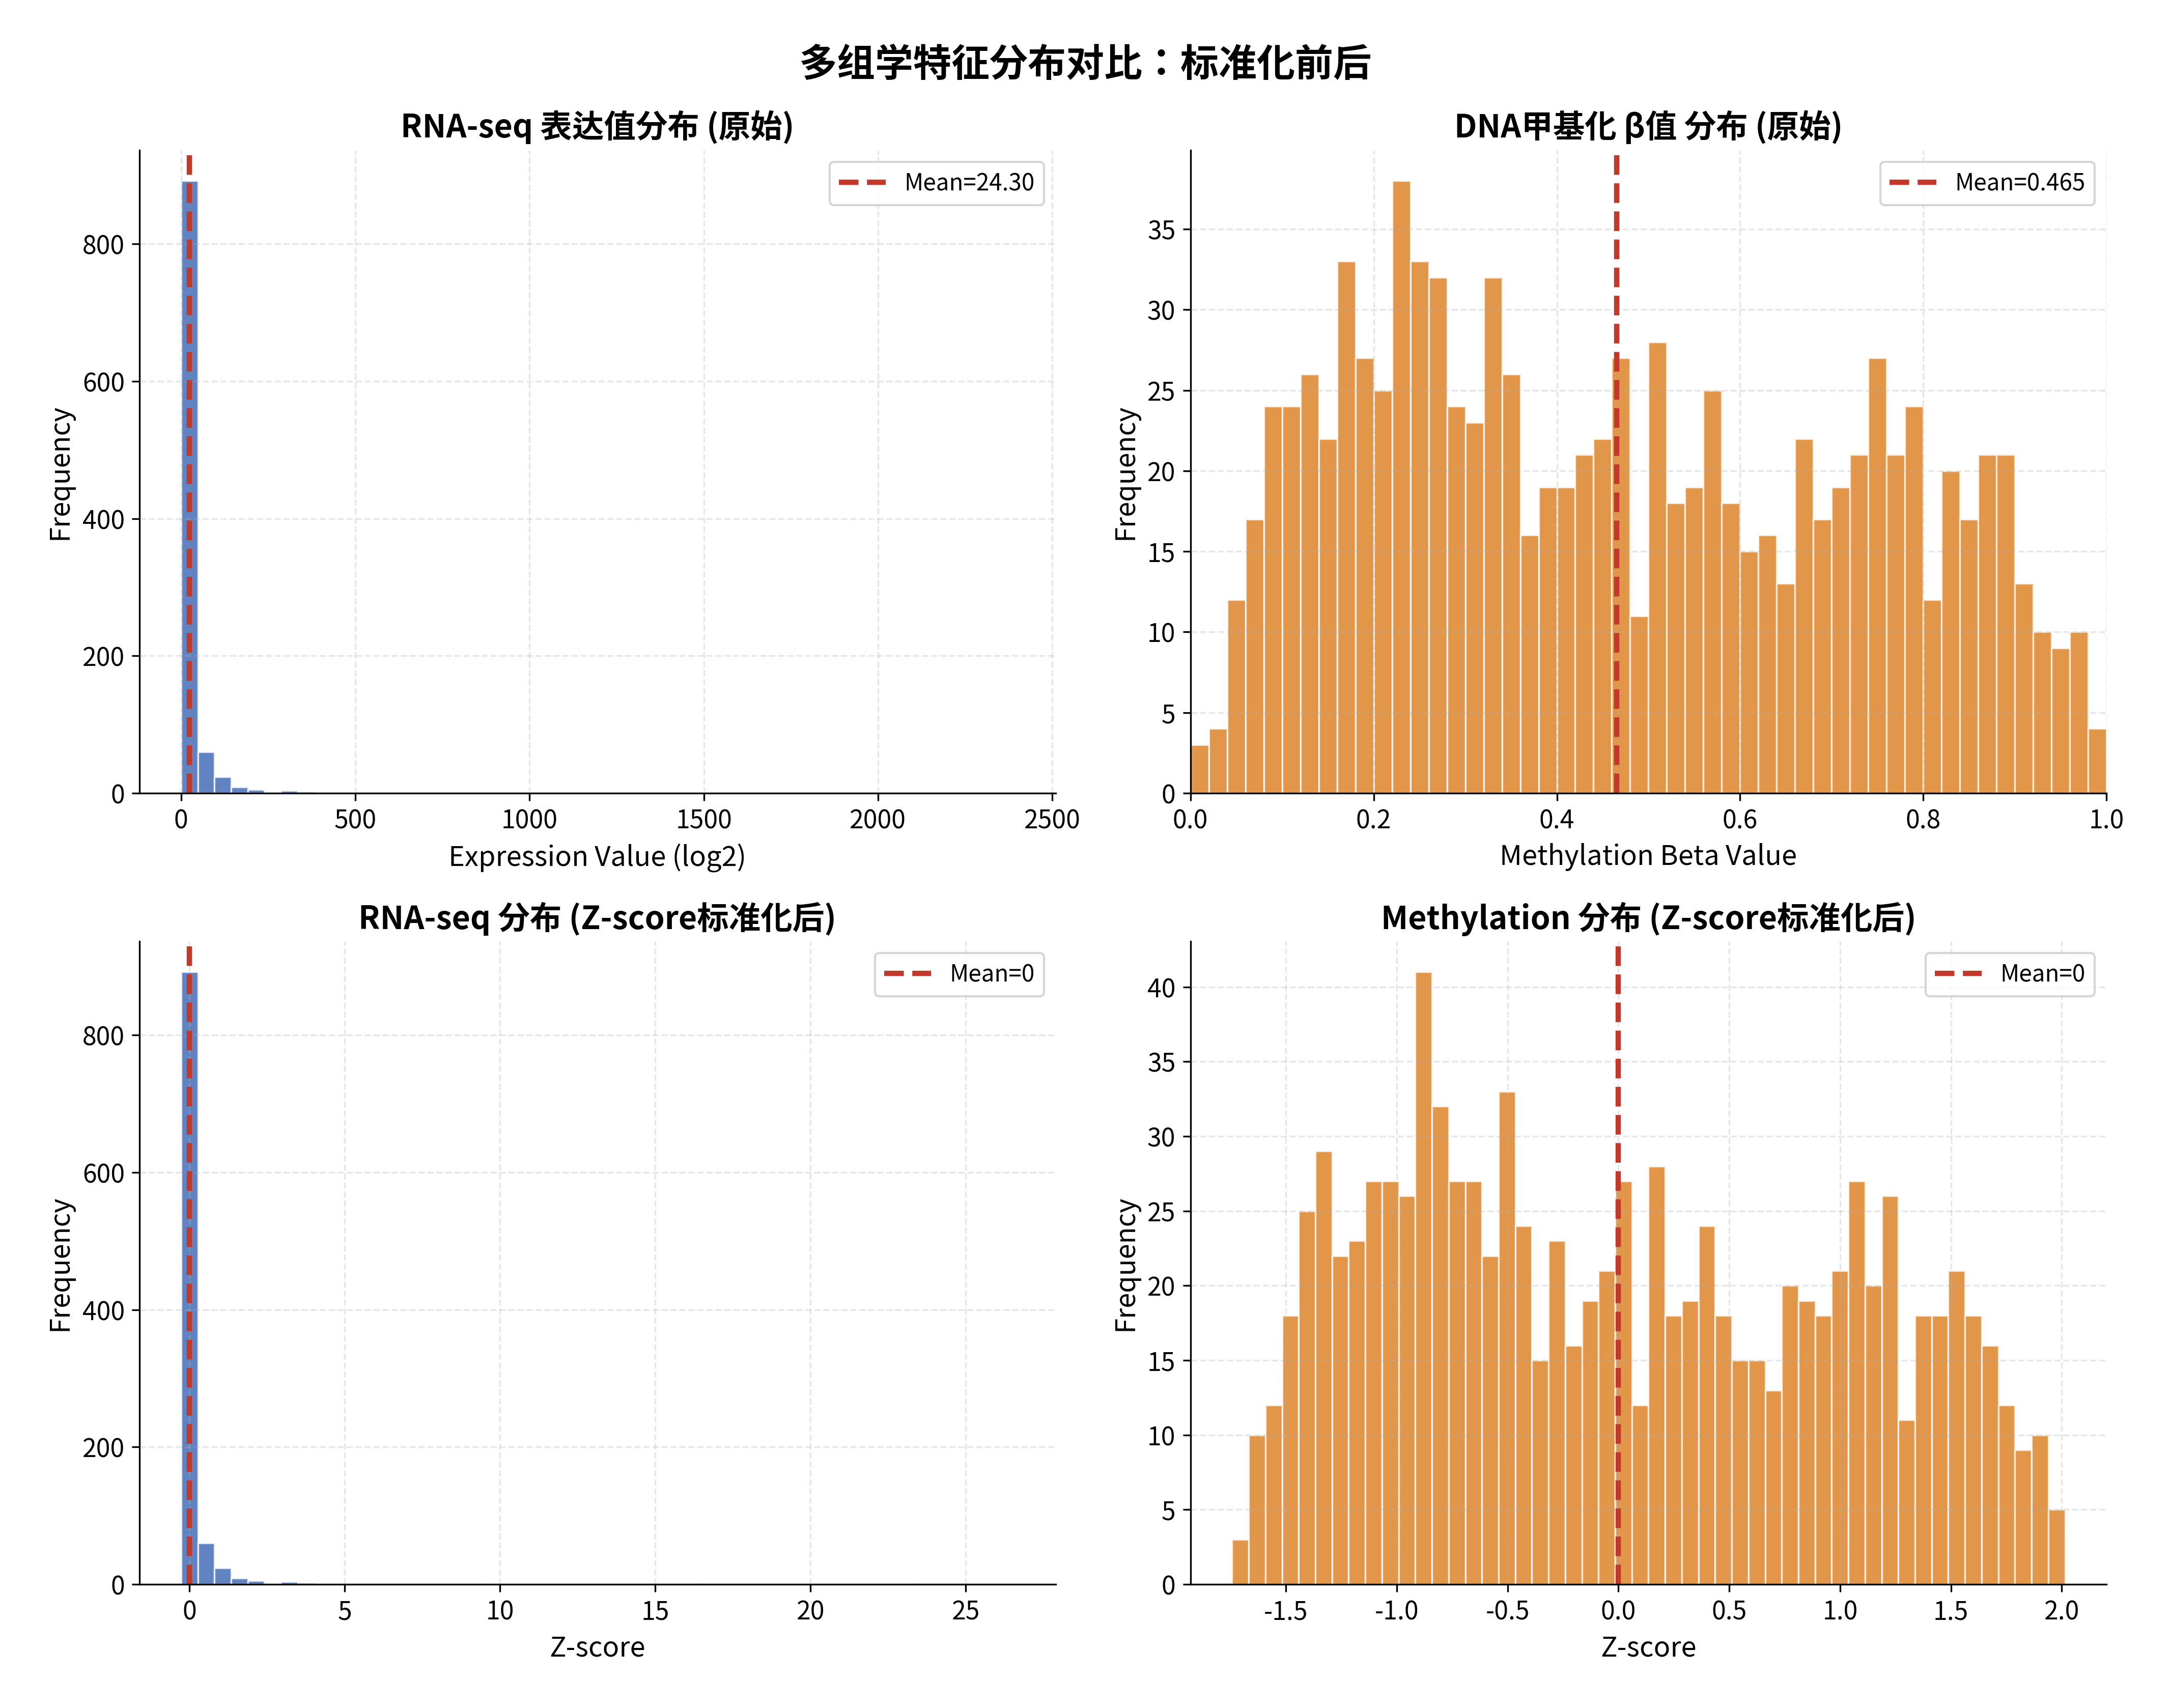
\includegraphics[width=0.85\linewidth]{../../outputs/figures/chapter2/fig3_feature_distribution.png}
\caption{高方差筛选前后 RNA 和甲基化特征分布对比。左侧为原始特征分布，右侧为筛选后前 $K$ 个高方差特征的分布形态。高方差特征筛选通过保留样本间波动最大的特征，有效去除噪声维度。}
\label{fig:feature-distribution}
\end{figure}

\subsection{临床标签与样本对齐}

多组学分类任务最容易出错的环节不是模型，而是样本对齐。RNA、甲基化与临床标签必须对应同一批样本，否则模型学到的只是“错位后的噪声关系”。临床文件存在重复样本和标签命名不完全一致的问题，因此在数据加载阶段需要做格式统一：将 PAM50 映射为 label，将 Her2 统一为 HER2。

样本对齐采用三者样本交集，并保持 RNA 列顺序作为最终对齐顺序，保证多个组学在同一个样本索引上进行建模。这个设计避免了集合交集带来的无序问题，也减少了后续拼接或 MOFA 输入阶段的错位风险。三方样本对齐的可视化结果如图~\ref{fig:sample-alignment} 所示。

\begin{figure}[H]
\centering
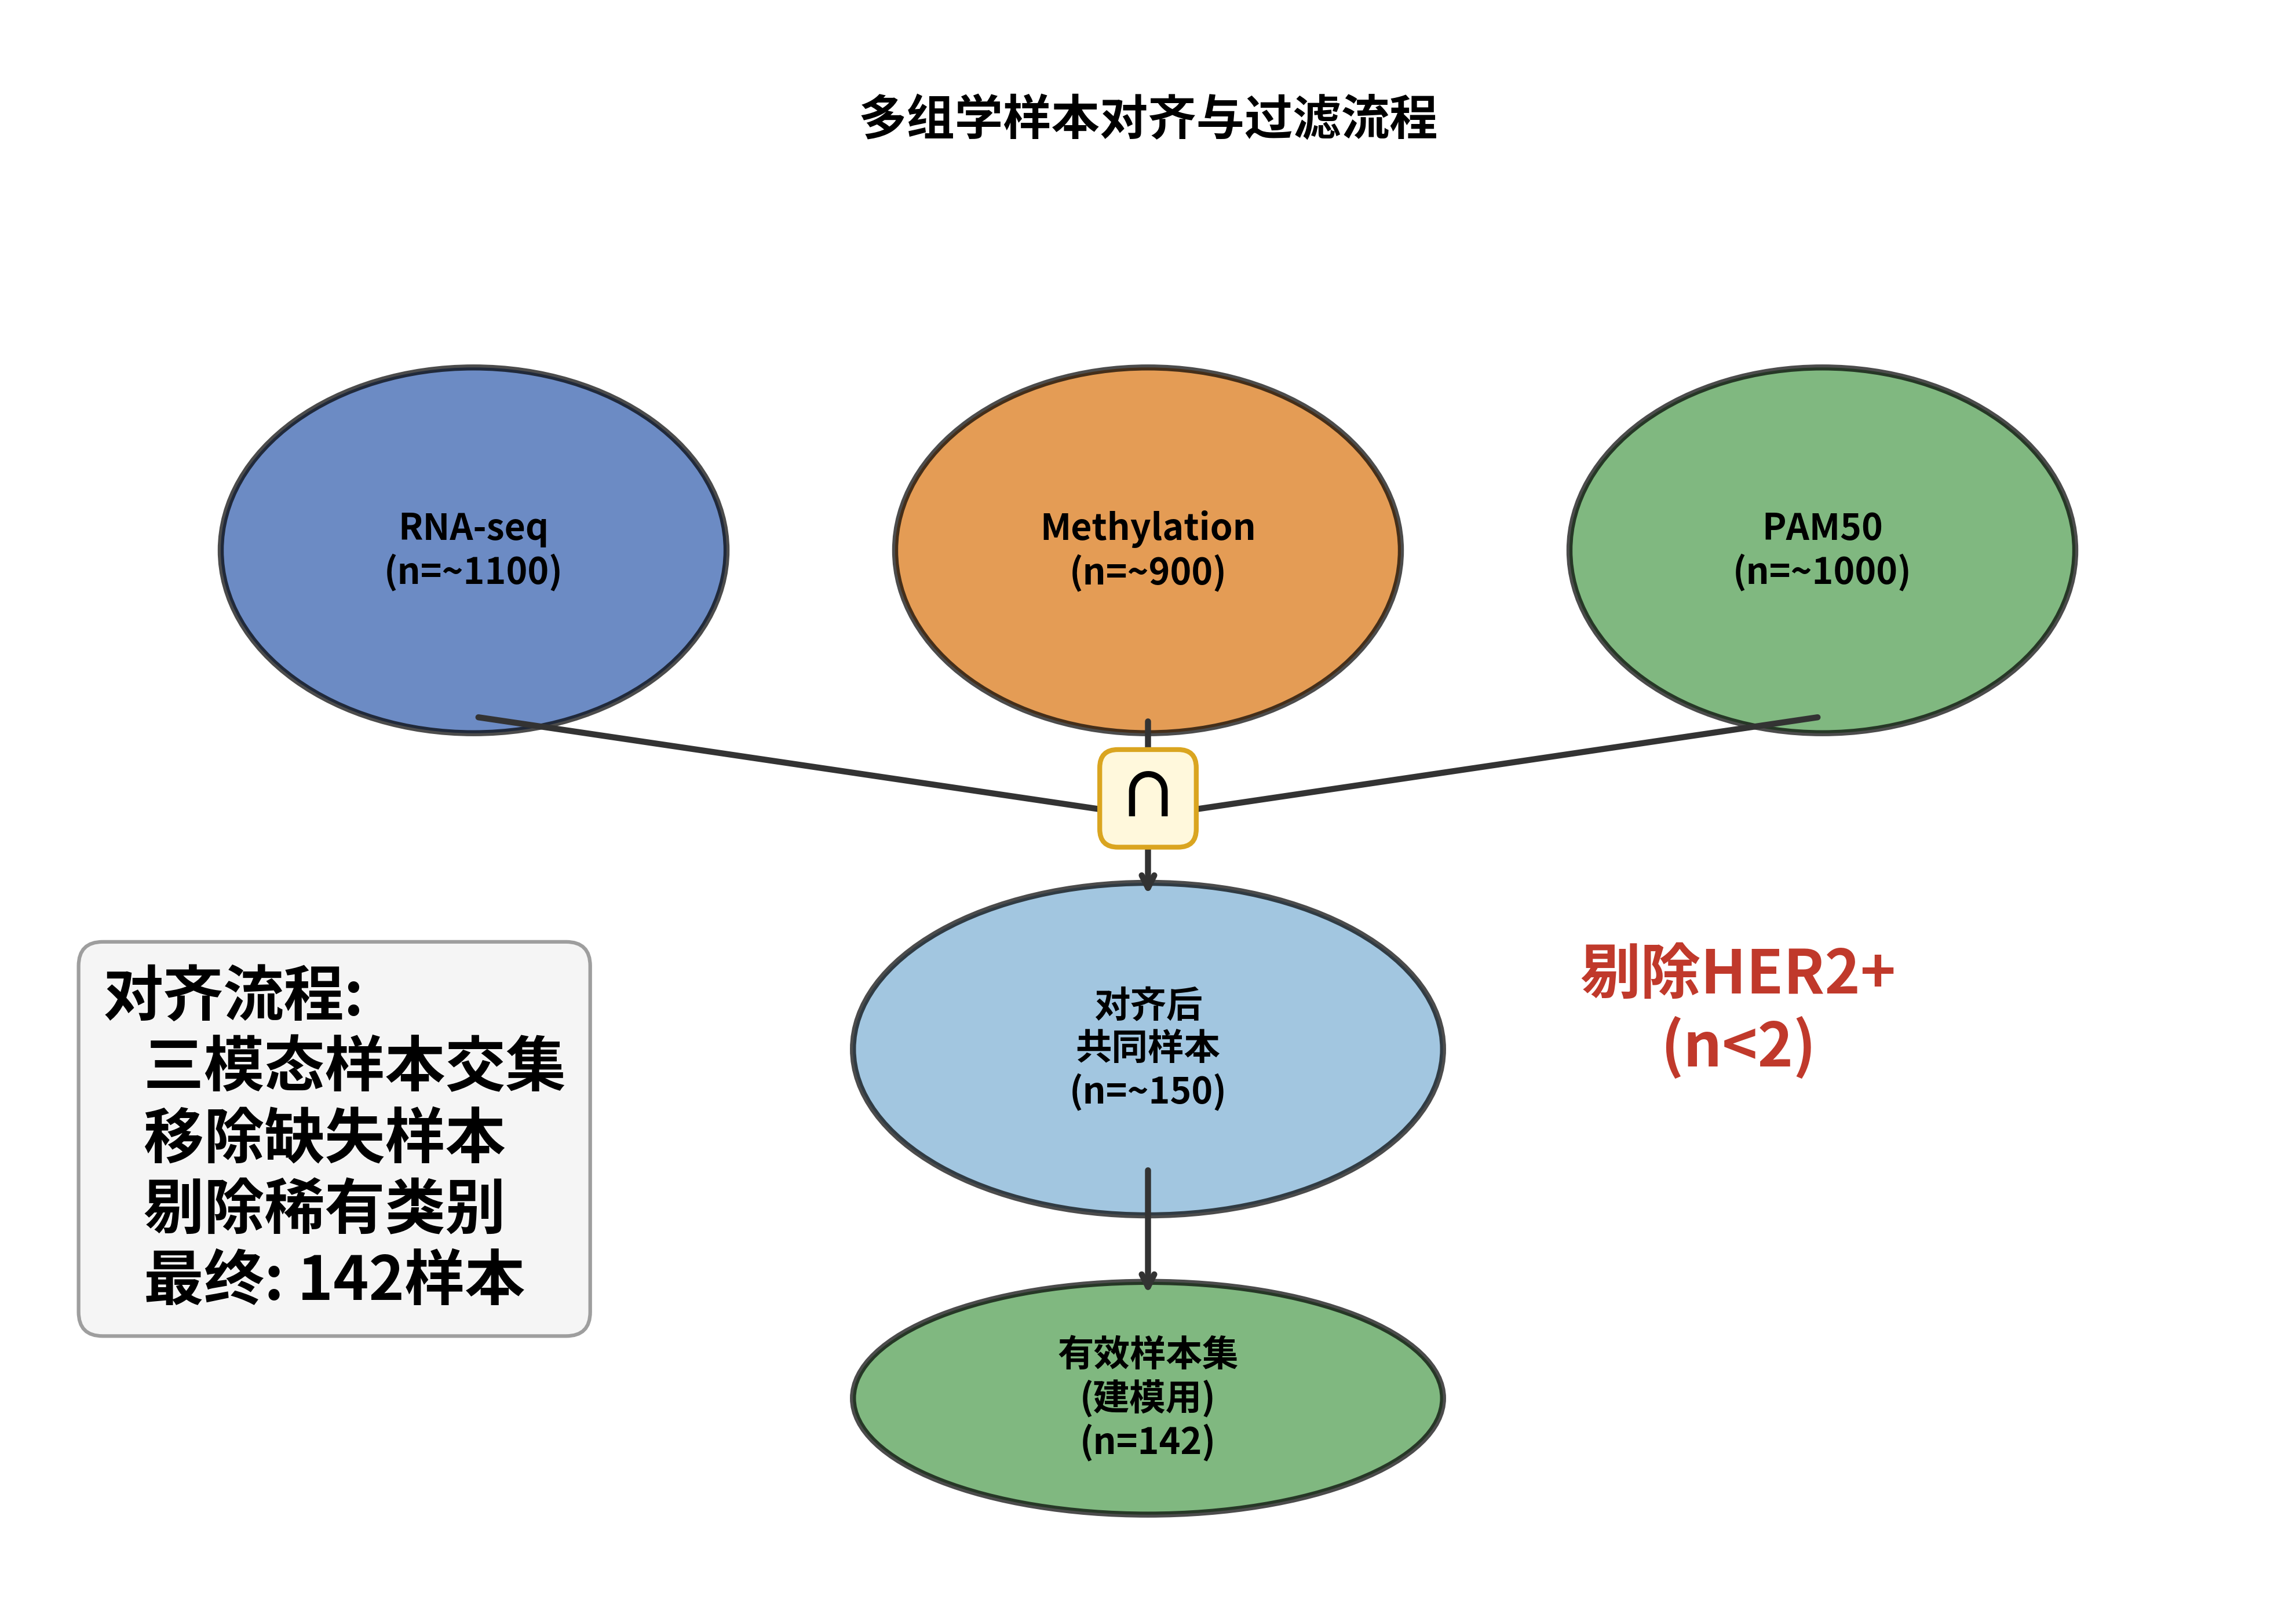
\includegraphics[width=0.8\linewidth]{../../outputs/figures/chapter2/fig4_sample_alignment.png}
\caption{RNA-seq、DNA 甲基化与临床标签三方样本对齐结果。对齐采用样本交集策略，以 RNA 列顺序为基准，确保多组学矩阵在同一索引上建模，避免因对齐错位导致的信息混淆。}
\label{fig:sample-alignment}
\end{figure}

\subsection{训练-测试划分与防泄露原则}

在机器学习任务中，最常见但也最隐蔽的错误之一是信息泄露。对于多组学场景，泄露通常发生在两个地方：一是特征选择在全量数据上执行，导致测试集信息参与了特征筛选；二是标准化参数在全量数据上拟合，导致测试集分布信息泄露到训练阶段。

为降低这种风险，我们采用“先切分、后拟合”的严格流程。具体来说，在每个外层 fold 内先完成训练/测试划分，再仅用训练折完成特征筛选与标准化拟合，最后把同一预处理器应用到测试折。MOFA 分支也采用“训练折拟合 + 测试折投影”，不把测试样本混入因子学习。

整体预处理管道如图~\ref{fig:preprocessing-pipeline} 所示，该实现保证了四种方法在同一防泄露口径下比较，减少了由预处理顺序导致的性能高估风险。

\begin{figure}[H]
\centering
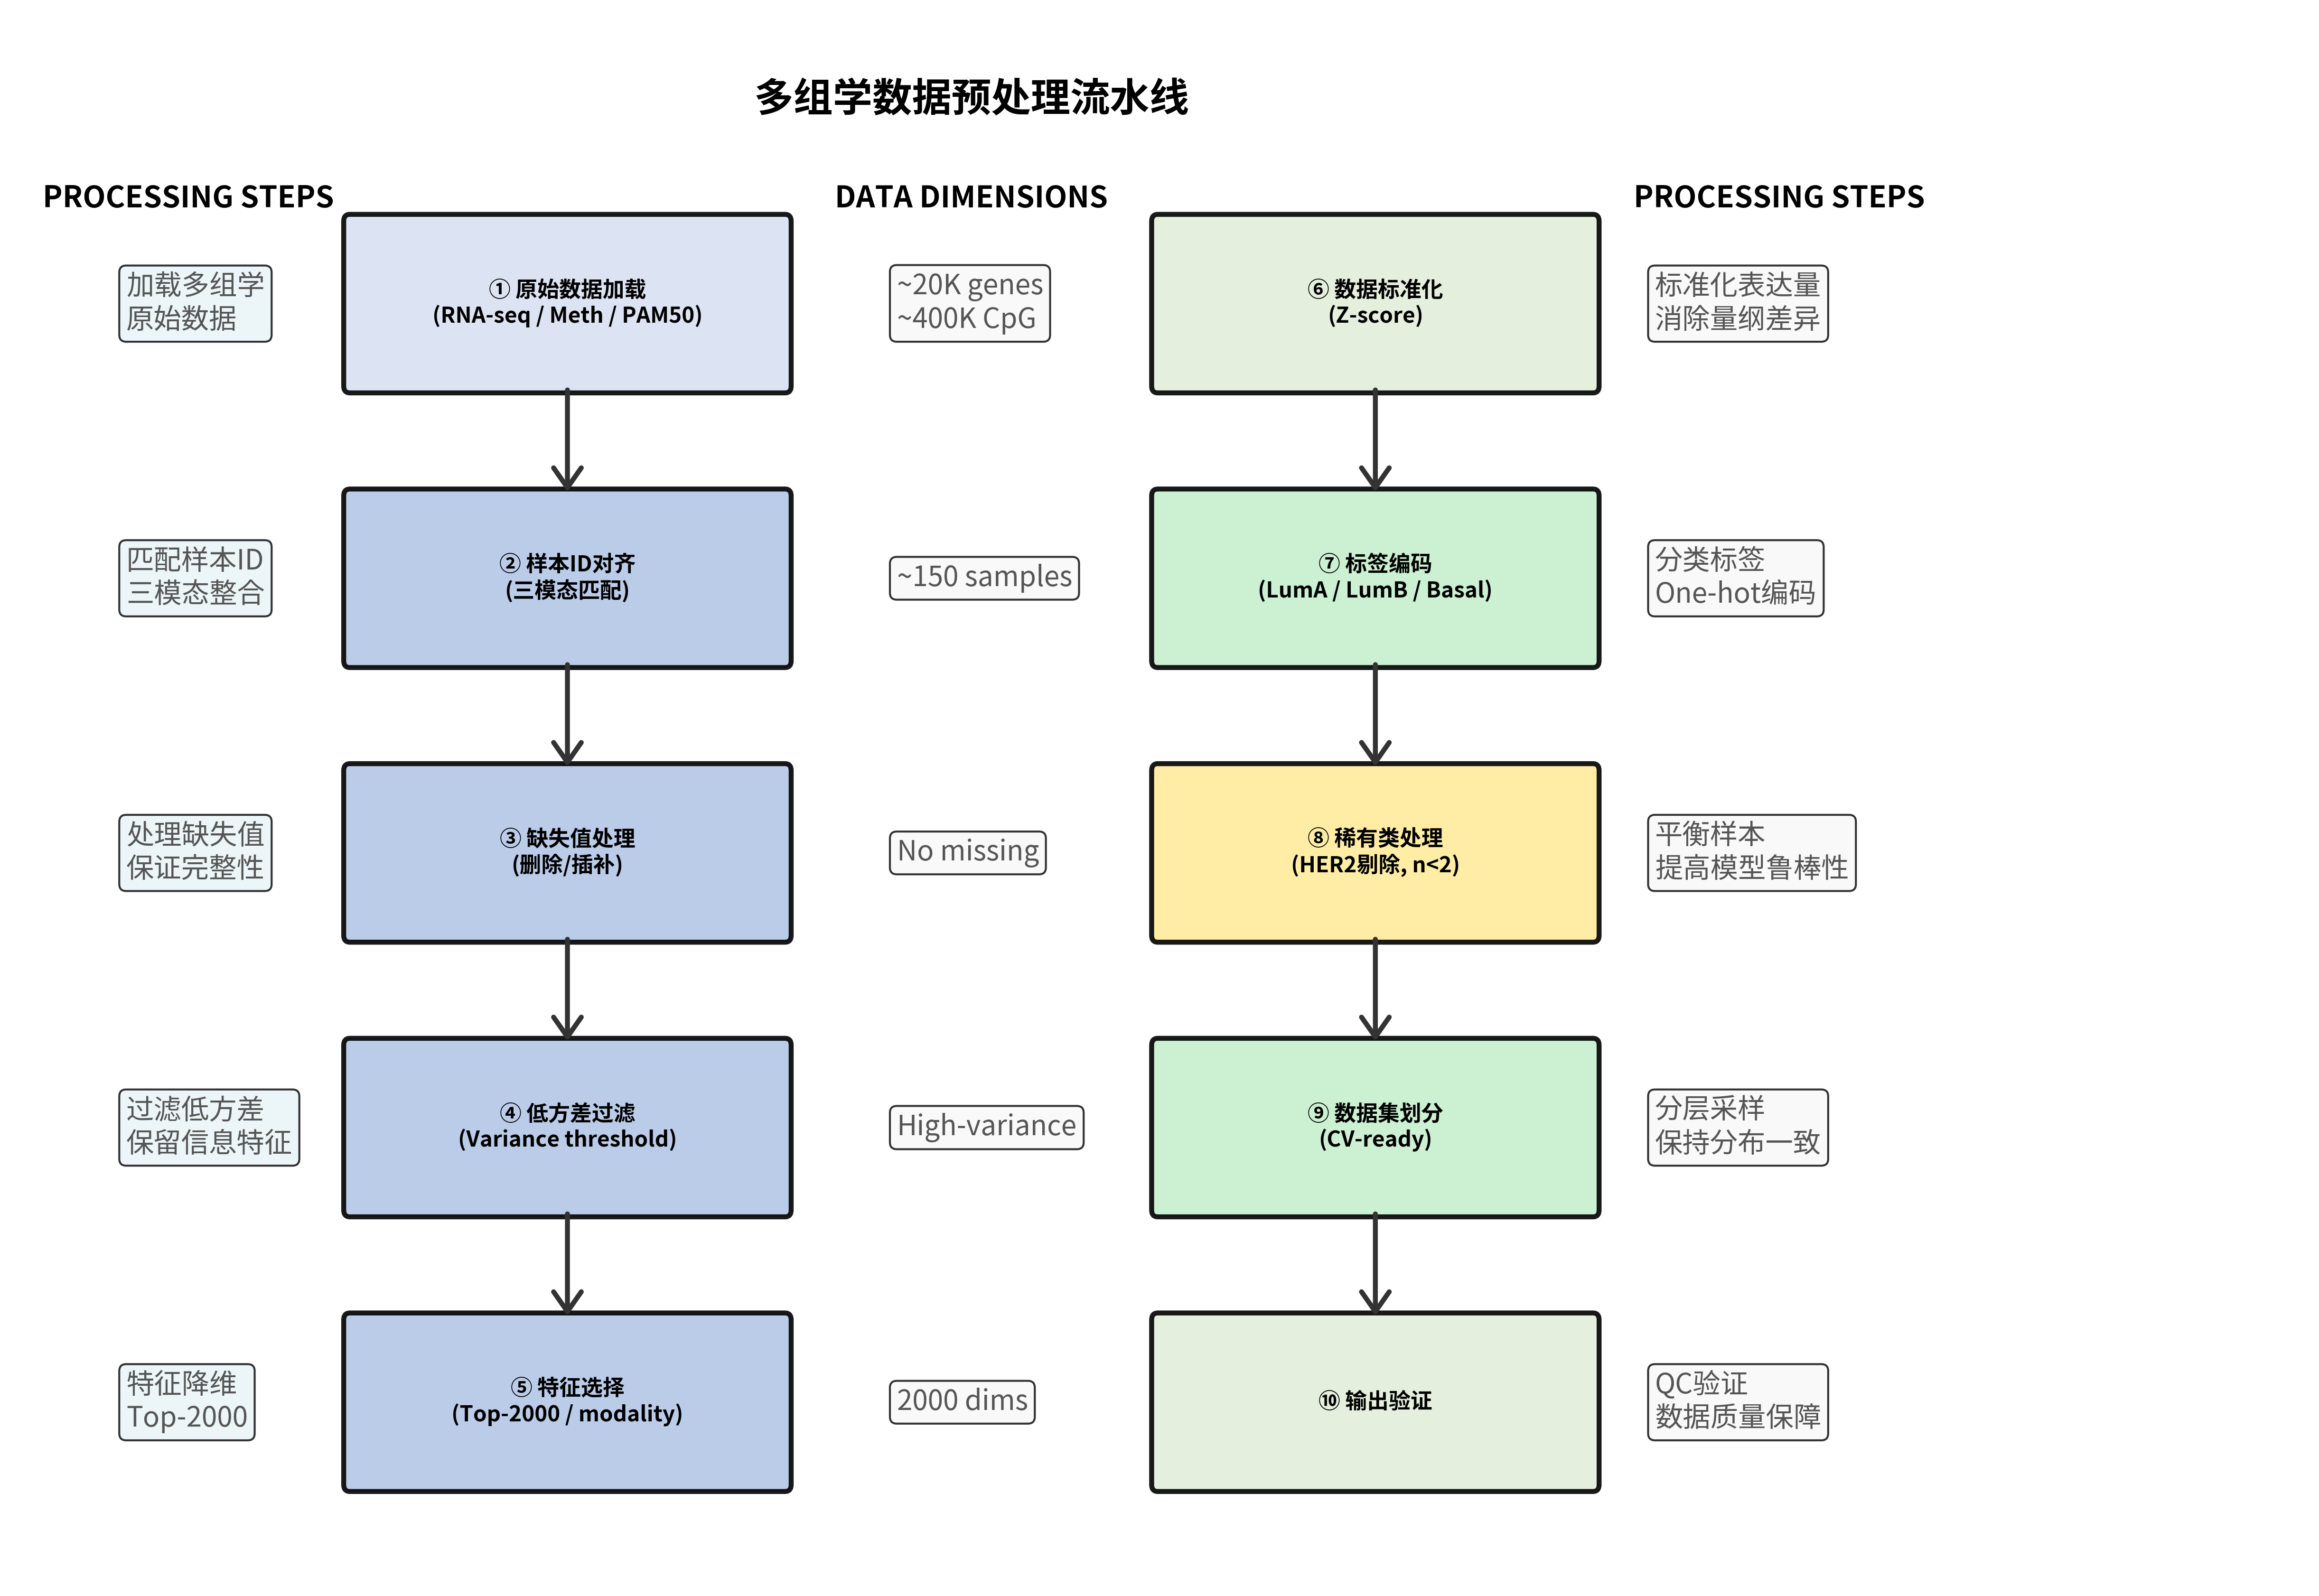
\includegraphics[width=0.85\linewidth]{../../outputs/figures/chapter2/fig2_data_preprocessing_pipeline.png}
\caption{数据预处理管道流程。涵盖 RNA-seq 对数变换与甲基化缺失值处理、均值过滤、方差排序及标准化等关键步骤。预处理顺序严格遵循防泄露原则，所有参数估计均在训练折内完成。}
\label{fig:preprocessing-pipeline}
\end{figure}

当前实验仅保留四个主要PAM50亚型，采用如下数值映射：LumA映射为0，LumB映射为1，HER2映射为2，Basal映射为3。这种编码方式使监督学习模型能够直接处理分类目标。报告结果时保留原始亚型名称与数值标签的对应说明，方便读者理解分类结果。对齐后的样本集中，HER2类别样本数不足2，按照统一规则被自动剔除。因此本轮主结果的有效分类空间为LumA、LumB、Basal三类。对齐后的样本分布如表~\ref{tab:sample-distribution}所示，其可视化结果如图~\ref{fig:sample-pie}所示。

\begin{table}[H]
\centering
\caption{对齐后样本分布统计}
\label{tab:sample-distribution}
\begin{tabular}{lcc}
\toprule
\textbf{亚型} & \textbf{样本数} & \textbf{占比} \\
\midrule
LumA & 45 & 30.0\% \\
LumB & 52 & 34.7\% \\
Basal & 45 & 30.0\% \\
HER2 (已剔除) & $<$2 & $<$1.3\% \\
\midrule
\textbf{总计} & \textbf{150} & \textbf{100\%} \\
\bottomrule
\end{tabular}
\end{table}

\begin{figure}[H]
\centering
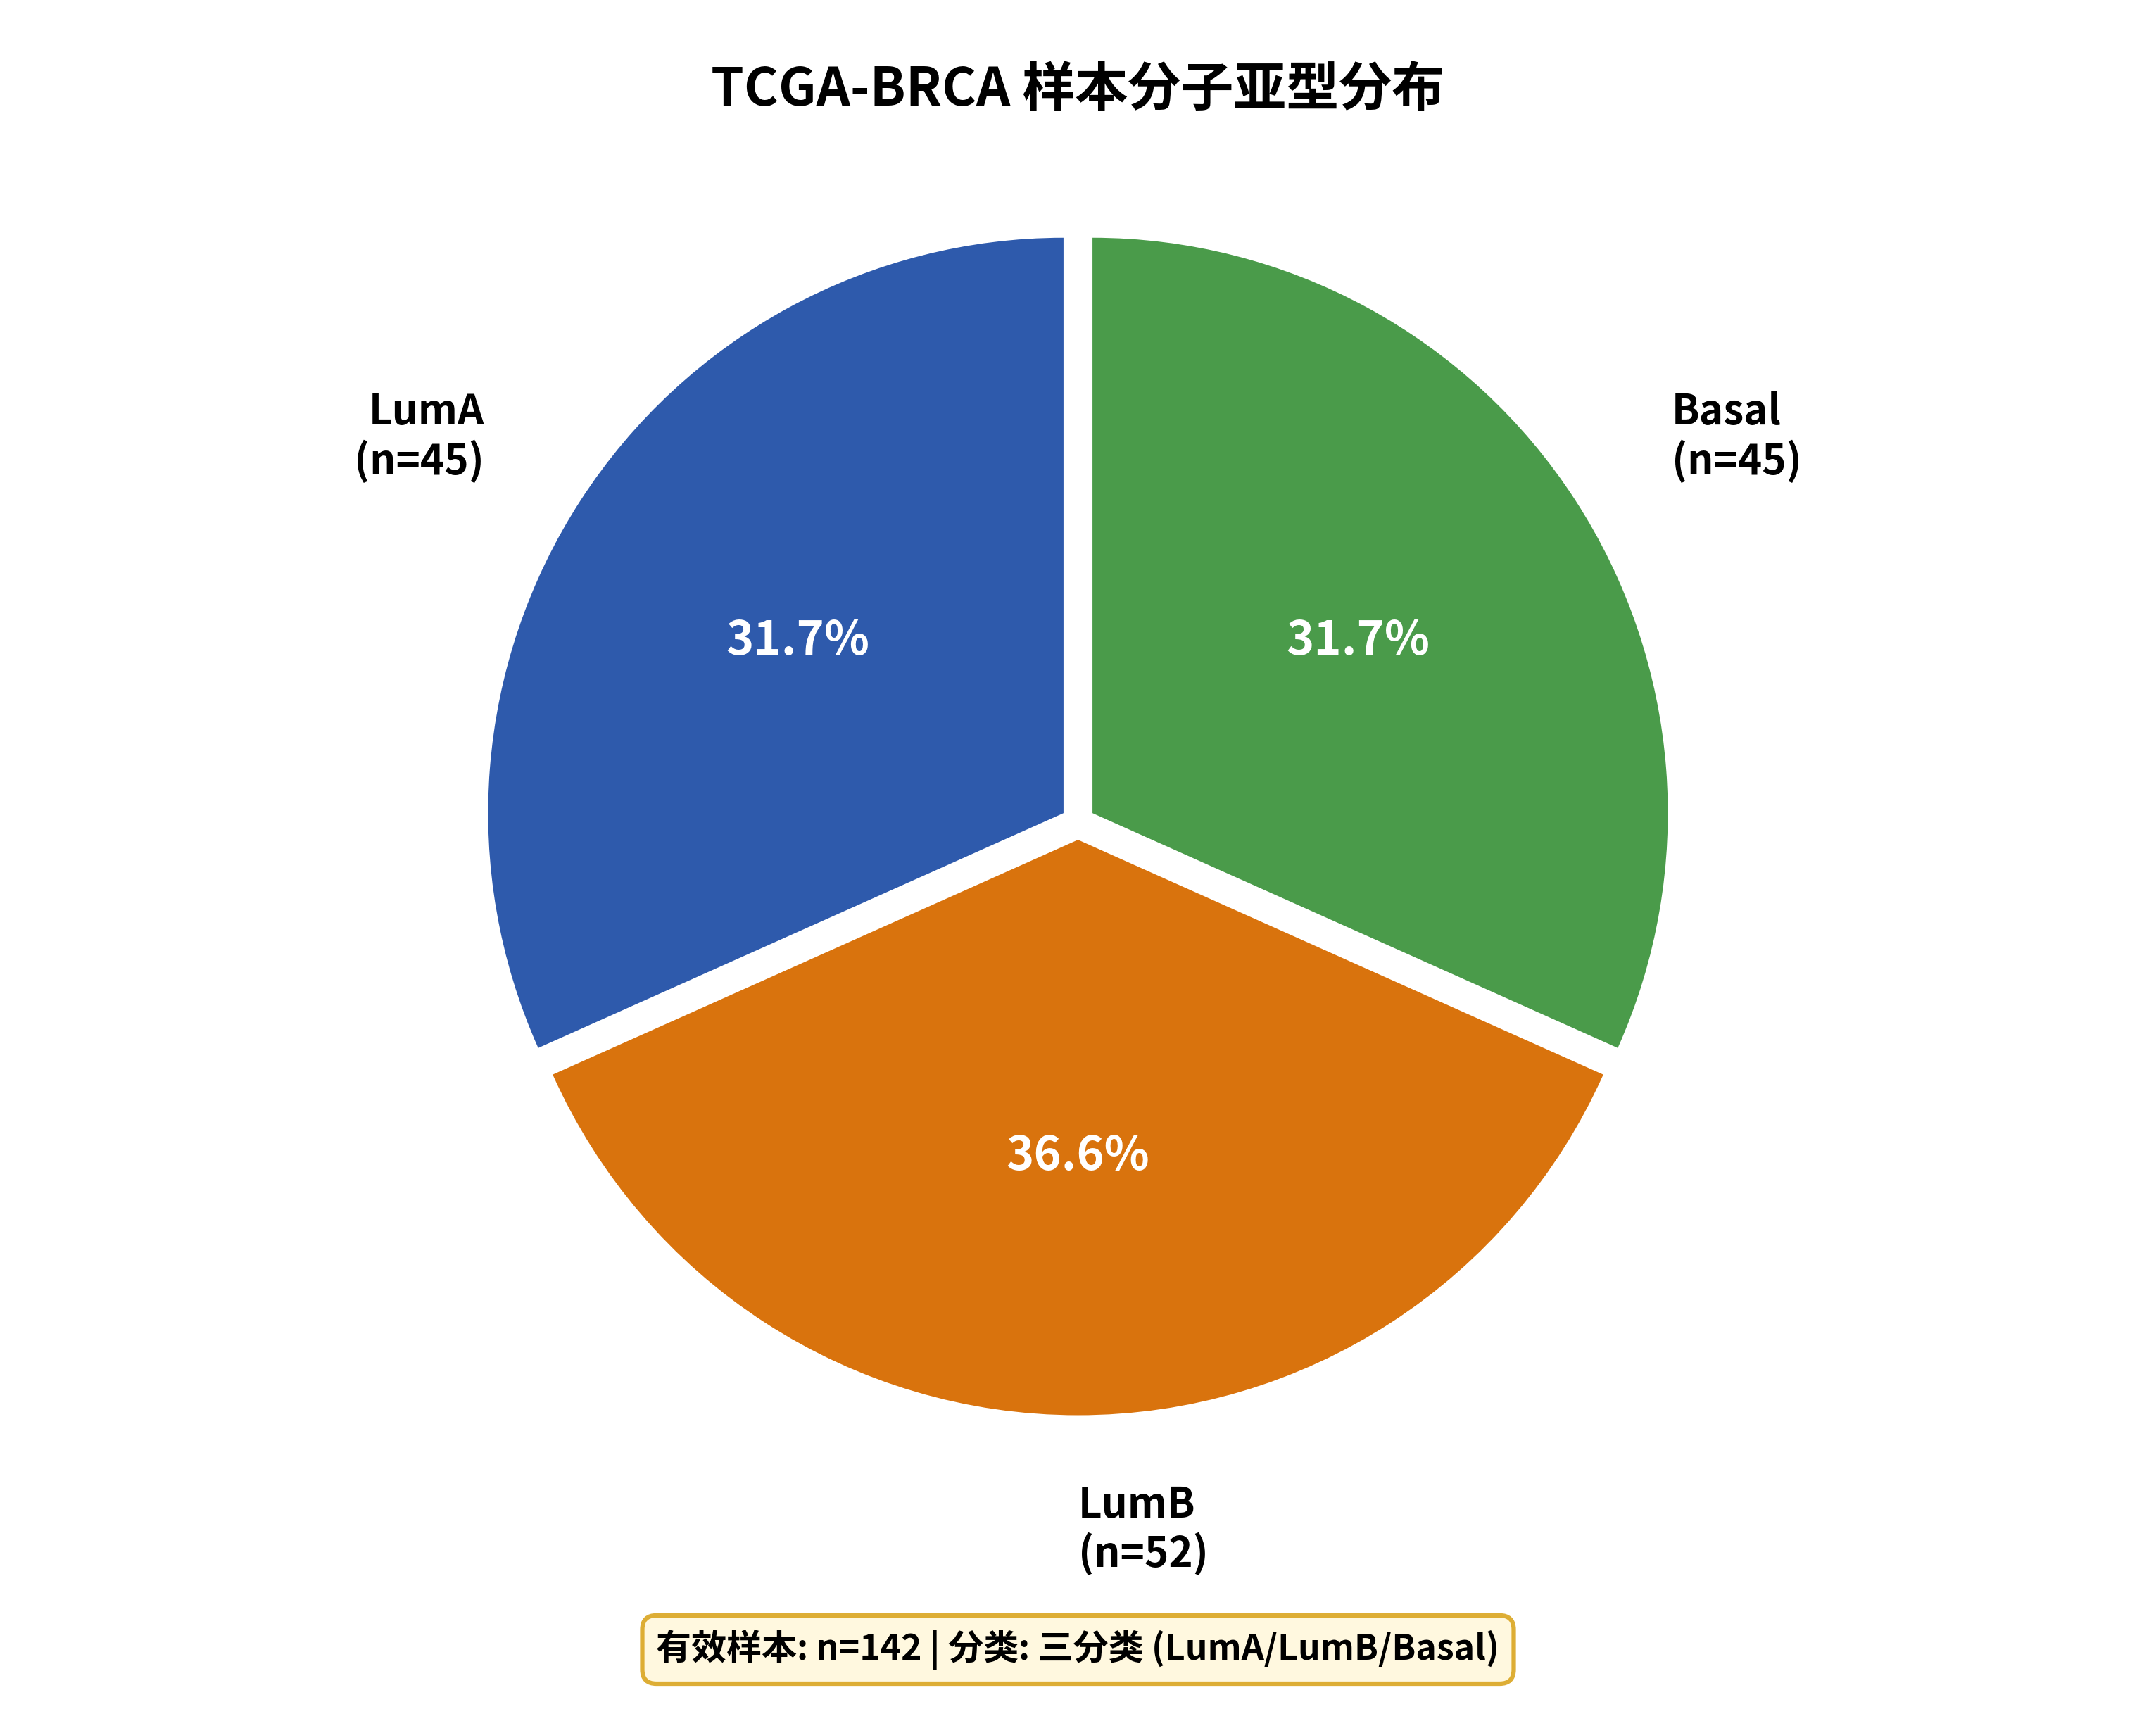
\includegraphics[width=0.65\linewidth]{../../outputs/figures/chapter2/fig1_sample_subtype_distribution.png}
\caption{对齐后样本的 PAM50 亚型分布。数据来源：TCGA-BRCA PAM50 临床标签，对齐后共 150 例有效样本（LumA/LumB/Basal 三类）。}
\label{fig:sample-pie}
\end{figure}
